\documentclass{homework}
% \usepackage{lua-visual-debug}
\usepackage{graphicx}
\usepackage{float}
\usepackage{minted}
\usepackage{subfig}
\usepackage[a4paper, total={6in, 8.8in}]{geometry}

\title{Practice \#2}
\subject{CS341 Introduction to Computer Networks}
\studentid{20170058}
\name{Keonwoo Kim}
\date{\today}

\AtBeginEnvironment{minted}{\singlespacing\fontsize{8}{12}\selectfont}
\newminted{latex}{breaklines=true,breaksymbolleft={}}
\usemintedstyle{manni}
\setminted{bgcolor=white!95!black}
\setmintedinline{fontsize=\small}

\begin{document}
\maketitle

\vspace*{-4em}


\begin{figure}[H]
  \centering
  \vspace*{-3.5em}
  \hspace*{-0.13\textwidth}\subfloat[client]{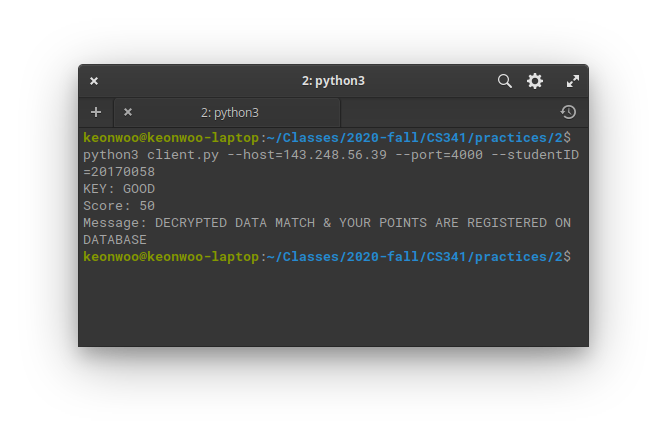
\includegraphics[width=0.7\textwidth]{client}}
  \subfloat[server]{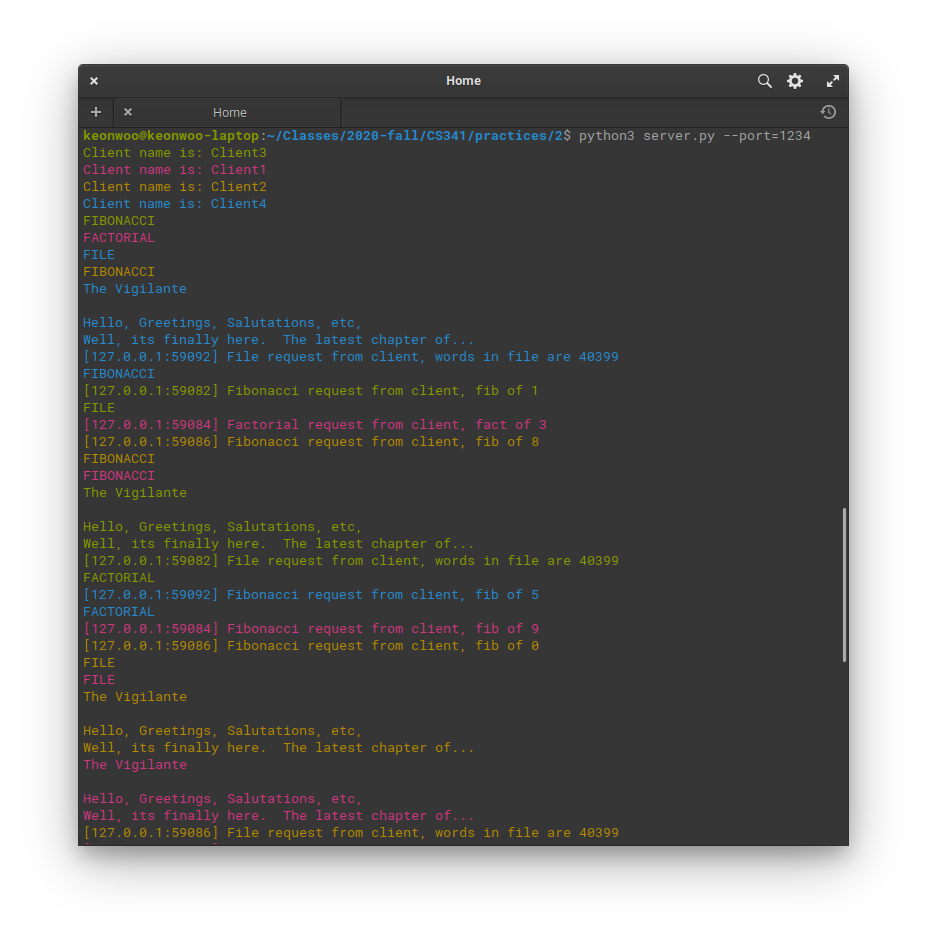
\includegraphics[width=0.5\textwidth]{server}}
\end{figure}

\section{Task 1}

The following is the code of the file \mintinline{text}{client.py}, with detailed and descriptive comments added. Only central implementations are shown below, and others are hidden in the file \mintinline{text}{client.py}.

\begin{minted}[fontsize=\footnotesize]{python}
# client.py
# [...]
def get_checksum(flag, keyword, sid, length, data):
    # split the message and data (with proper zero padding),
    # sum them, get the 1's complement by XOR with 0xffff,
    # and finally change the endianness
    bytes_array = split_bytes(struct.pack(
        '!H4sII', flag, keyword, sid, length) + data + zero_padding(len(data)))
    return change_endianness(one_complement_sum(bytes_array) ^ 0xffff)
# [...]
def en_or_decrypt(key, data):
    # do the XOR cipher,
    # by repeatedly applying `en_or_decrypt_four_bytes` below to each 4 bytes
    postproc = ""
    while len(postproc) < len(data):
        postproc += en_or_decrypt_four_bytes(key, data[len(postproc):len(postproc) + 4])
    return postproc
def en_or_decrypt_four_bytes(key, data):
    # make the key and the data into int's,
    # do XOR, and re-pack into bytes.
    # if the length of `data` is less than 4,
    # cut the result accordingly (to make the result has the same length as `data`)
    unpacked_key = struct.unpack("!I", key)[0]
    four_bytes = struct.unpack("!I", (data + b"\x00\x00\x00")[0:4])[0]
    postproc = struct.pack("!I", unpacked_key ^ four_bytes).decode()
    return postproc[0:len(data)]
# [...]
def run(host, port, sid):
    with socket.socket(socket.AF_INET, socket.SOCK_STREAM) as s:
        # connect to the given host and port
        s.connect((host, port))
        # make and send the initial packet
        initial_packet = pack_data(1, b"sbmt", sid, b"")
        s.send(initial_packet)

        while True:
            msg = s.recv(10000)
            # if the header is arrived incompletely, wait again
            if len(msg) < 16:
                continue
            # get the complete header
            (flag, checksum, keyword, sid_, length) = struct.unpack(
                '!HH4sII', msg[0:16])
            # receive until the claimed length is reached
            while len(msg) < length:
                msg += s.recv(length - len(msg))

            # assert the checksum matches
            data = msg[16:]
            assert get_checksum(flag, keyword, sid_, length, data) == checksum

            # grading message -> terminate
            if keyword == b"FAIL" or keyword == b"GOOD":
                print("KEY:", keyword.decode())
                print("Score:", sid_)
                print("Message:", msg[16:].decode())
                break

            # elsewise, decrypt the message and send it
            decrypted = en_or_decrypt(keyword, data)
            packet = pack_data(flag, keyword, sid_, decrypted.encode())
            s.send(packet)
# [...]
\end{minted}

\section{Task 2}

The following is the code of the file \mintinline{text}{server.py}, with detailed and descriptive comments added. Only central implementations are shown below, and others are hidden in the file \mintinline{text}{server.py}.

\newpage

\begin{minted}[fontsize=\footnotesize]{python}
# server.py
# [...]
def thread_function(connection, client_address, name, uid, index):
    # The function which threads will execute
    connection.settimeout(120)
    connection.send(str(uid).encode())
    
    while True:
        # Get the message type: one of FIBONACCI, FACTORIAL, FILE, and COMPLETE
        msg_type = connection.recv(MAX_BYTES).decode()
        thread_print(index, msg_type)

        if msg_type == "FIBONACCI":
            # Get n from the client message
            n = int(connection.recv(MAX_BYTES).decode())
            thread_print(index, "[%s:%d] Fibonacci request from client, fib of %d" %
                         (client_address[0], client_address[1], n))
            connection.send(answer(fib(n), uid))
        elif msg_type == "FACTORIAL":
            # Get n from the client message
            n = int(connection.recv(MAX_BYTES).decode())
            thread_print(index, "[%s:%d] Factorial request from client, fact of %d" %
                         (client_address[0], client_address[1], n))
            connection.send(answer(fact(n), uid))
        elif msg_type == "FILE":
            # Get file length from the client message
            file_length = int(connection.recv(MAX_BYTES).decode())
            # Repeat to receive the client message until the text has reached the claimed file length
            current_text = ""
            while len(current_text) < file_length:
                text = connection.recv(file_length).decode()
                current_text += text
            # [...]
            # The number of words in the text
            ans = len(current_text.split(" "))
            thread_print(index, "[%s:%d] File request from client, words in file are %d" %
                         (client_address[0], client_address[1], ans))
            connection.send(answer(ans, uid))
        elif msg_type == "COMPLETE":
            connection.close()
            break

def run(host, port):
    with socket.socket(socket.AF_INET, socket.SOCK_STREAM) as s:
        s.bind((host, port))
        s.listen()
        while True:
            # Accept the client connection
            connection, client_address = s.accept()
            # Receive the name of the client
            name = connection.recv(10000)
            name = name.decode()
            # [...]
            x = threading.Thread(target=thread_function, args=(
                connection, client_address, name, uid, index))
            x.start()
\end{minted}

\end{document}